\chapter{Discussion}\label{ch:Discussion}\addtocontents{lof}{\protect\contentsline{chapter}{\protect\numberline{\thechapter}Discussion}{}{}}
\newthought{Synopsis}\synopsisDiscussion

\section{Challenges and the Various Explored Approaches}
\subsection{Modelling Challenges}
\newthought{Mould Die Design}\\
The decision in the early stages of the project of working off of a pre-constructed anatomically accurate valve geometry spawned many issues; it didn't allow for feature interaction in SolidWorks, which prompted some very suboptimal prototyping choices that ended in a huge amount of time investment for an avenue that was eventually made obsolete upon later findings. The series of 2-stage epoxy moulds developed as discussed in \cref{fig:moulddie} had a 72 hour curing time, which made the turnaround for learnings very slow to implement and iterate.

This process became obsolete when the SolidWorks package being used was arbitrarily updated in later stages. It was discovered that the 'Segment Mesh' tool previously attempted to be used to convert the STL to a mesh body and then mesh body to solid part had been overhauled to allow more complex geometries to be segmented. On this discovery, the part was successfully converted to a solid body, which allowed for features like body subtraction to remove it from an encompassing cylindrical body as originally planned before encountering the bug, which was then split into what were the foundations of the final design press mould pieces.

From this point, further iterations of the press mould were exponentially quicker, taking only 4-5 hours, reducing the print-to-casting time by 95\%, and taking only 20 hours for finalised designs where print settings were maximised for quality and strength of the part.
\begin{figure}[H]
    \centering
    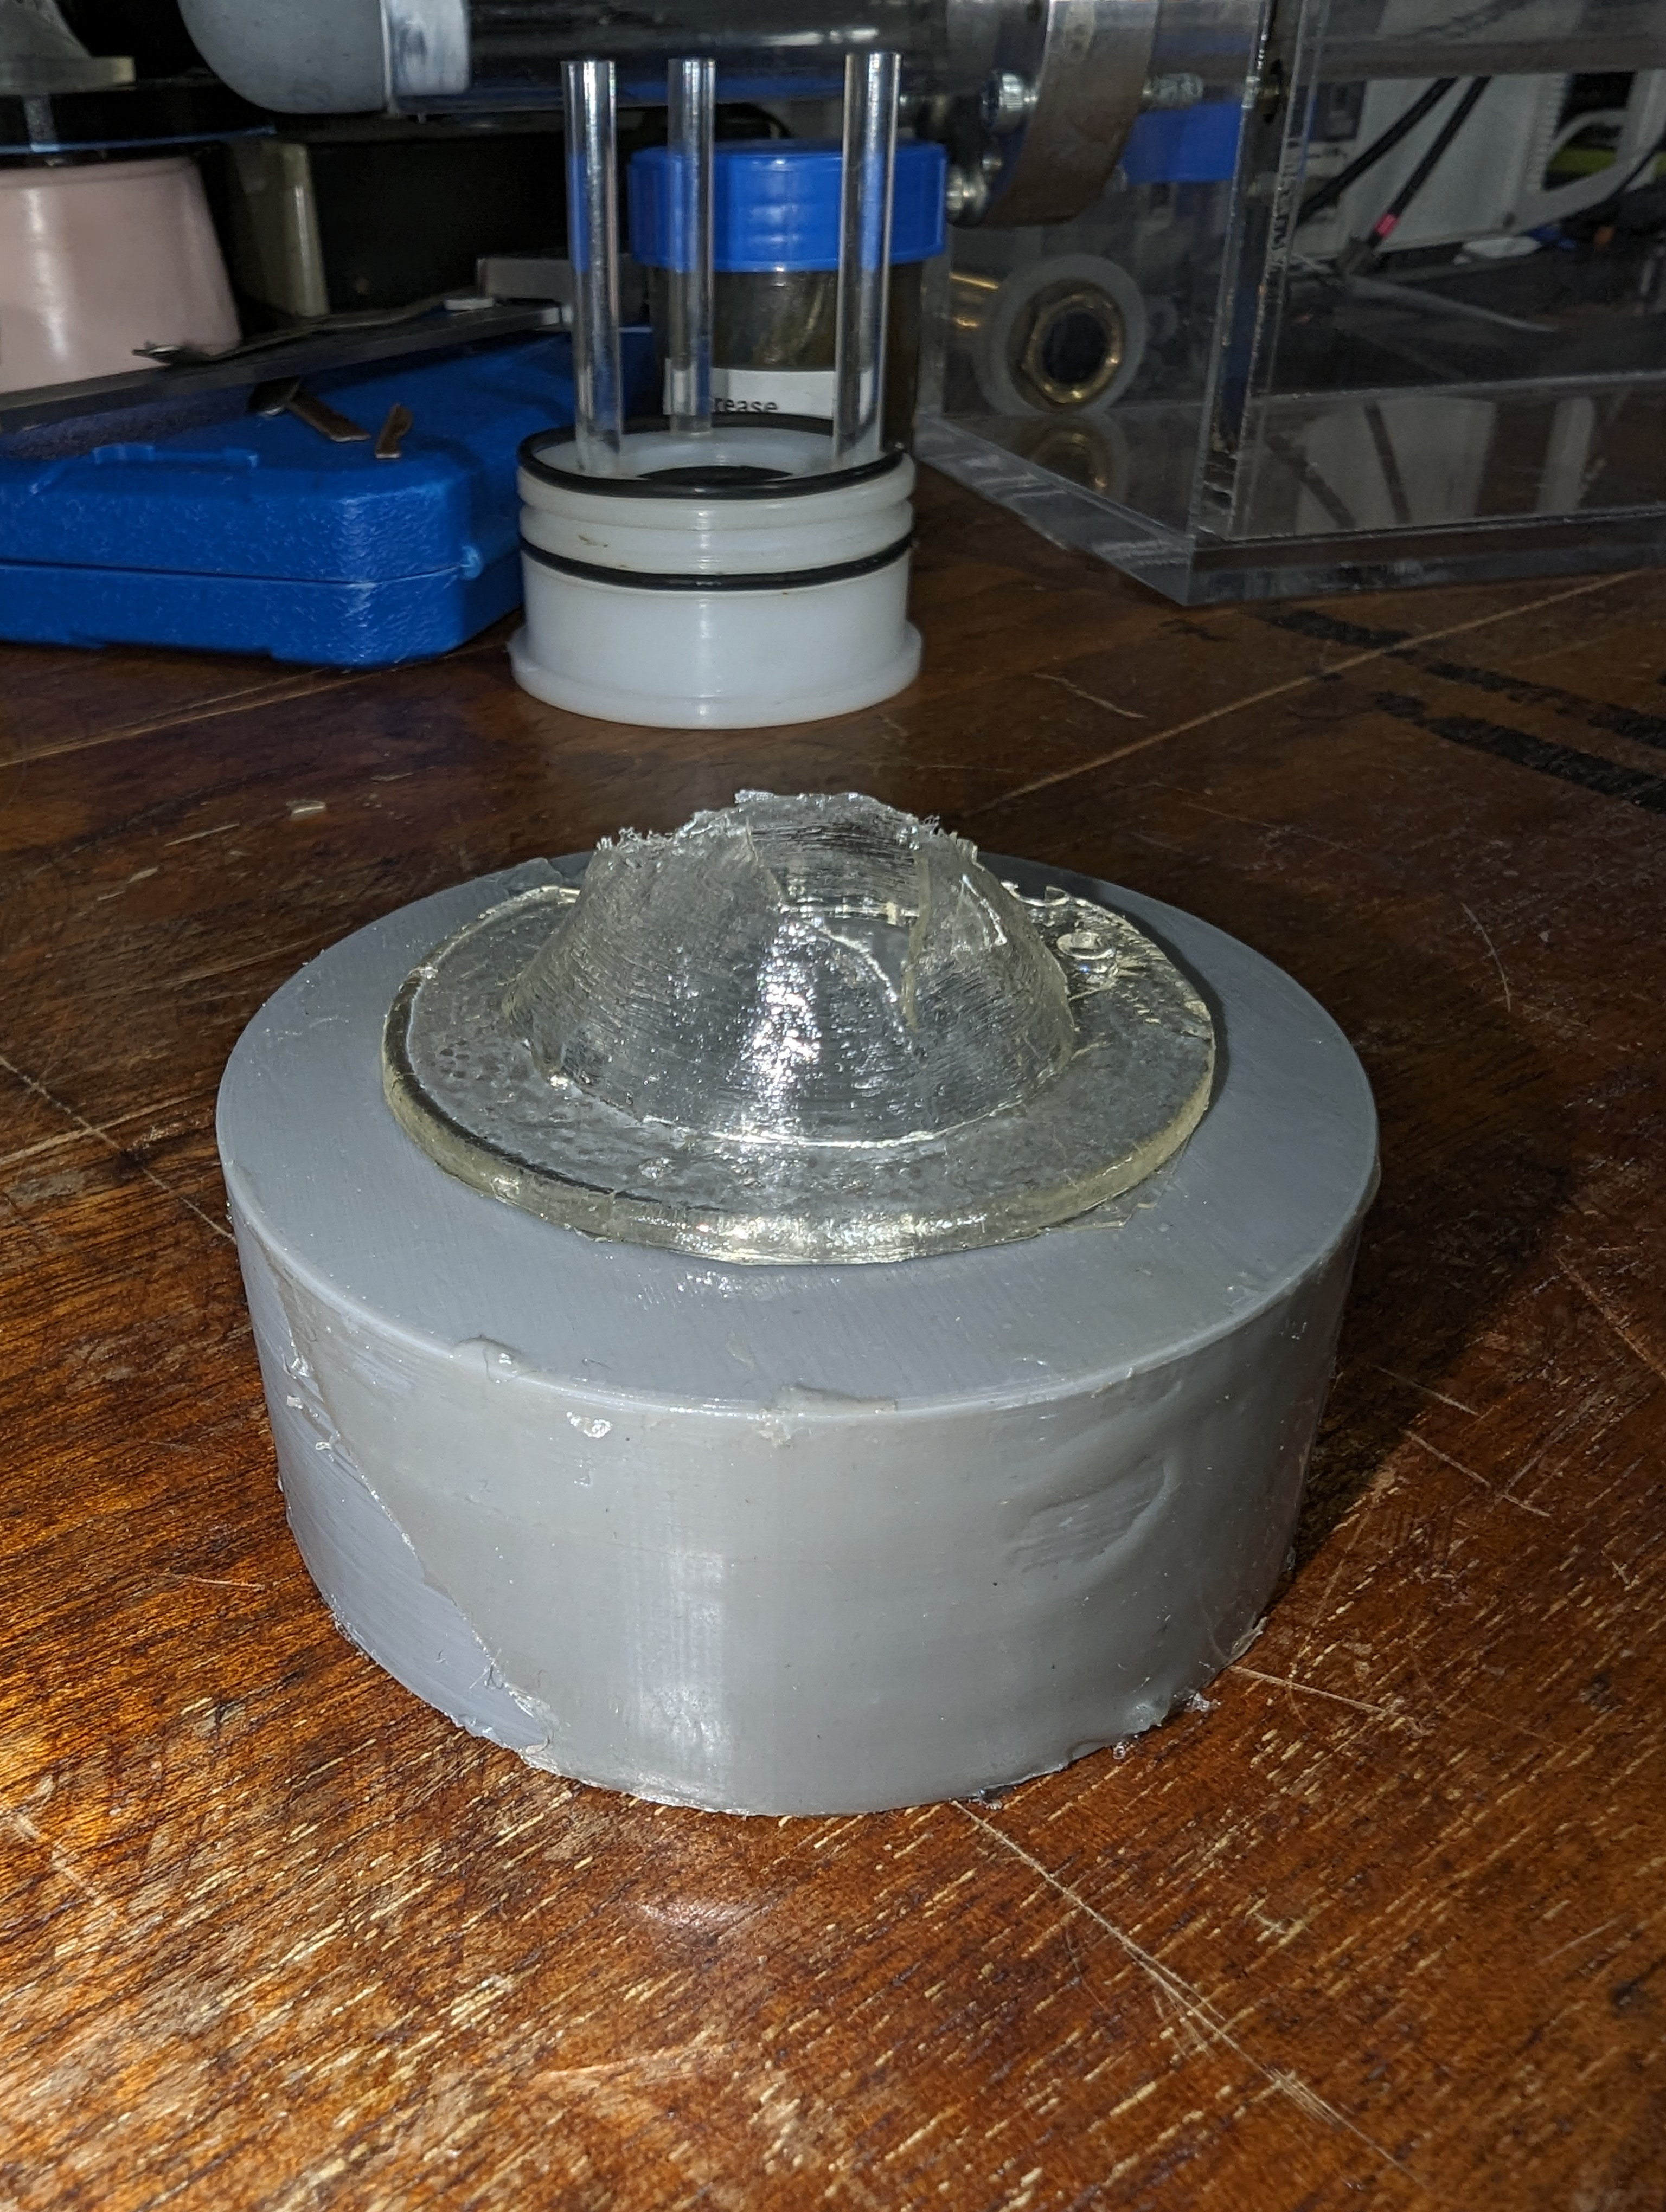
\includegraphics[width=0.75\textwidth]{figures/latercastnice.jpg}
    \caption{Final cast of anatomical valve}
    \label{fig:cast1}
\end{figure}

\newthought{Valve Design}\\
Another area that caused an excess of time consumption was the post-processing of the anatomical valve geometry, in becoming acquainted with STL modelling\sidenote{Software packages like Blender use mainly sculpting tools that are used to modify the surface as opposed traditional CAD programs like SolidWorks where parts are built up from a tree of features} on the various programs trialled throughout the study, the model was transferred across systems to utilise the different tools each had, for example, Blender had great sculpting tools but lacked simple geometry analysis which was required for monitoring the surface as the thickness was homogenised.

While Blender has the capability to manipulate shaders to render this kind of information, due to it being an open-source program, developing a custom shader for this was very complex and deemed not worth the time for other trialled programs like MeshMixer could suffice albeit added unnecessary steps. If further work was conducted with many patient-specific models being developed, it would be likely the most efficient option to develop a custom tool however.

\subsection{Manufacturing Challenges}

\newthought{Chordae Tendineae Prototyping}\\
The tendineae attachment to the leaflets was another highly contested and thought-out design factor. Balancing the rigidity that is added to the leaflets by some methods in attaching the nylon wire and the adhesion to the leaflet is very difficult; for the scope of this study it was found that B7000 adhesive worked well as the tendineae could be effectively attached with minimal disruption to the mechanics of the valve however this did add thickness to the leaflets which not only adds rigidity that hinders coaptation in experimental use but also brings many issues for potential computational simulations that could be conducted in tandem to a study of this nature.

Studies like \citeonly{karlExvivoInvitroDynamic2024} only published in the end stages of the study use a method of embedding their chordae tendineae within the leaflets, containing a medical gauze matrix, so that the tendineae do not detach under tensile forces like was seend in section:\cref{sec:Chord} with the embed tests. An approach like this could prove very effective in application to this study as it would simplify the manufacturing process in that the tendineae can be attached to the gauze matrix prior to \gls{PU} casting ensuring accurate and repeatable placement across multiple fabrications without any added thickness to the part.

\newthought{Valve Prototyping}\\
The prototyping conducted through the study for finalised parts, fixturing, and the experimental rig revealed a few key insights into the rapid prototyping landscape. For each print, the printer's configuration was tailored to the purpose of the parts being produced. Parts being made in early iterations were set to a faster infill and layer height setting, whereas finalised ideas were set to slower, higher resolution settings.

These dense high-definition settings needed for an accurate and rigid mould die had issues that took many iterations and failed prints to perfect. They often resulted in a large amount of stringing, a printing defect that was often not solvable via post-processing. To circumnavigate this the researchers in the UCD print lab were consulted. Tailored settings in Prusa Slicer were programmed for the geometry where the resulting gcode would stop the nozzle from crossing the perimeter of the valve moulds, retraction settings would stop the printer from leaving blobs of residue on the interior of the mould and z-axis seams were aligned to not interfere with the geometry.
\mynewline
In the earlier stages of the study, a resin \gls{SLA} printer was used to manufacture an anatomic model for the silicone mould method discussed in \cref{fig:silimould}, however, it was not feasible to develop further iterations from resin due to the printer being in a separate lab and having a much higher cost with proprietary resins. Two major benefits to \gls{SLA} printing are;

\begin{figure}[H]
    \centering
    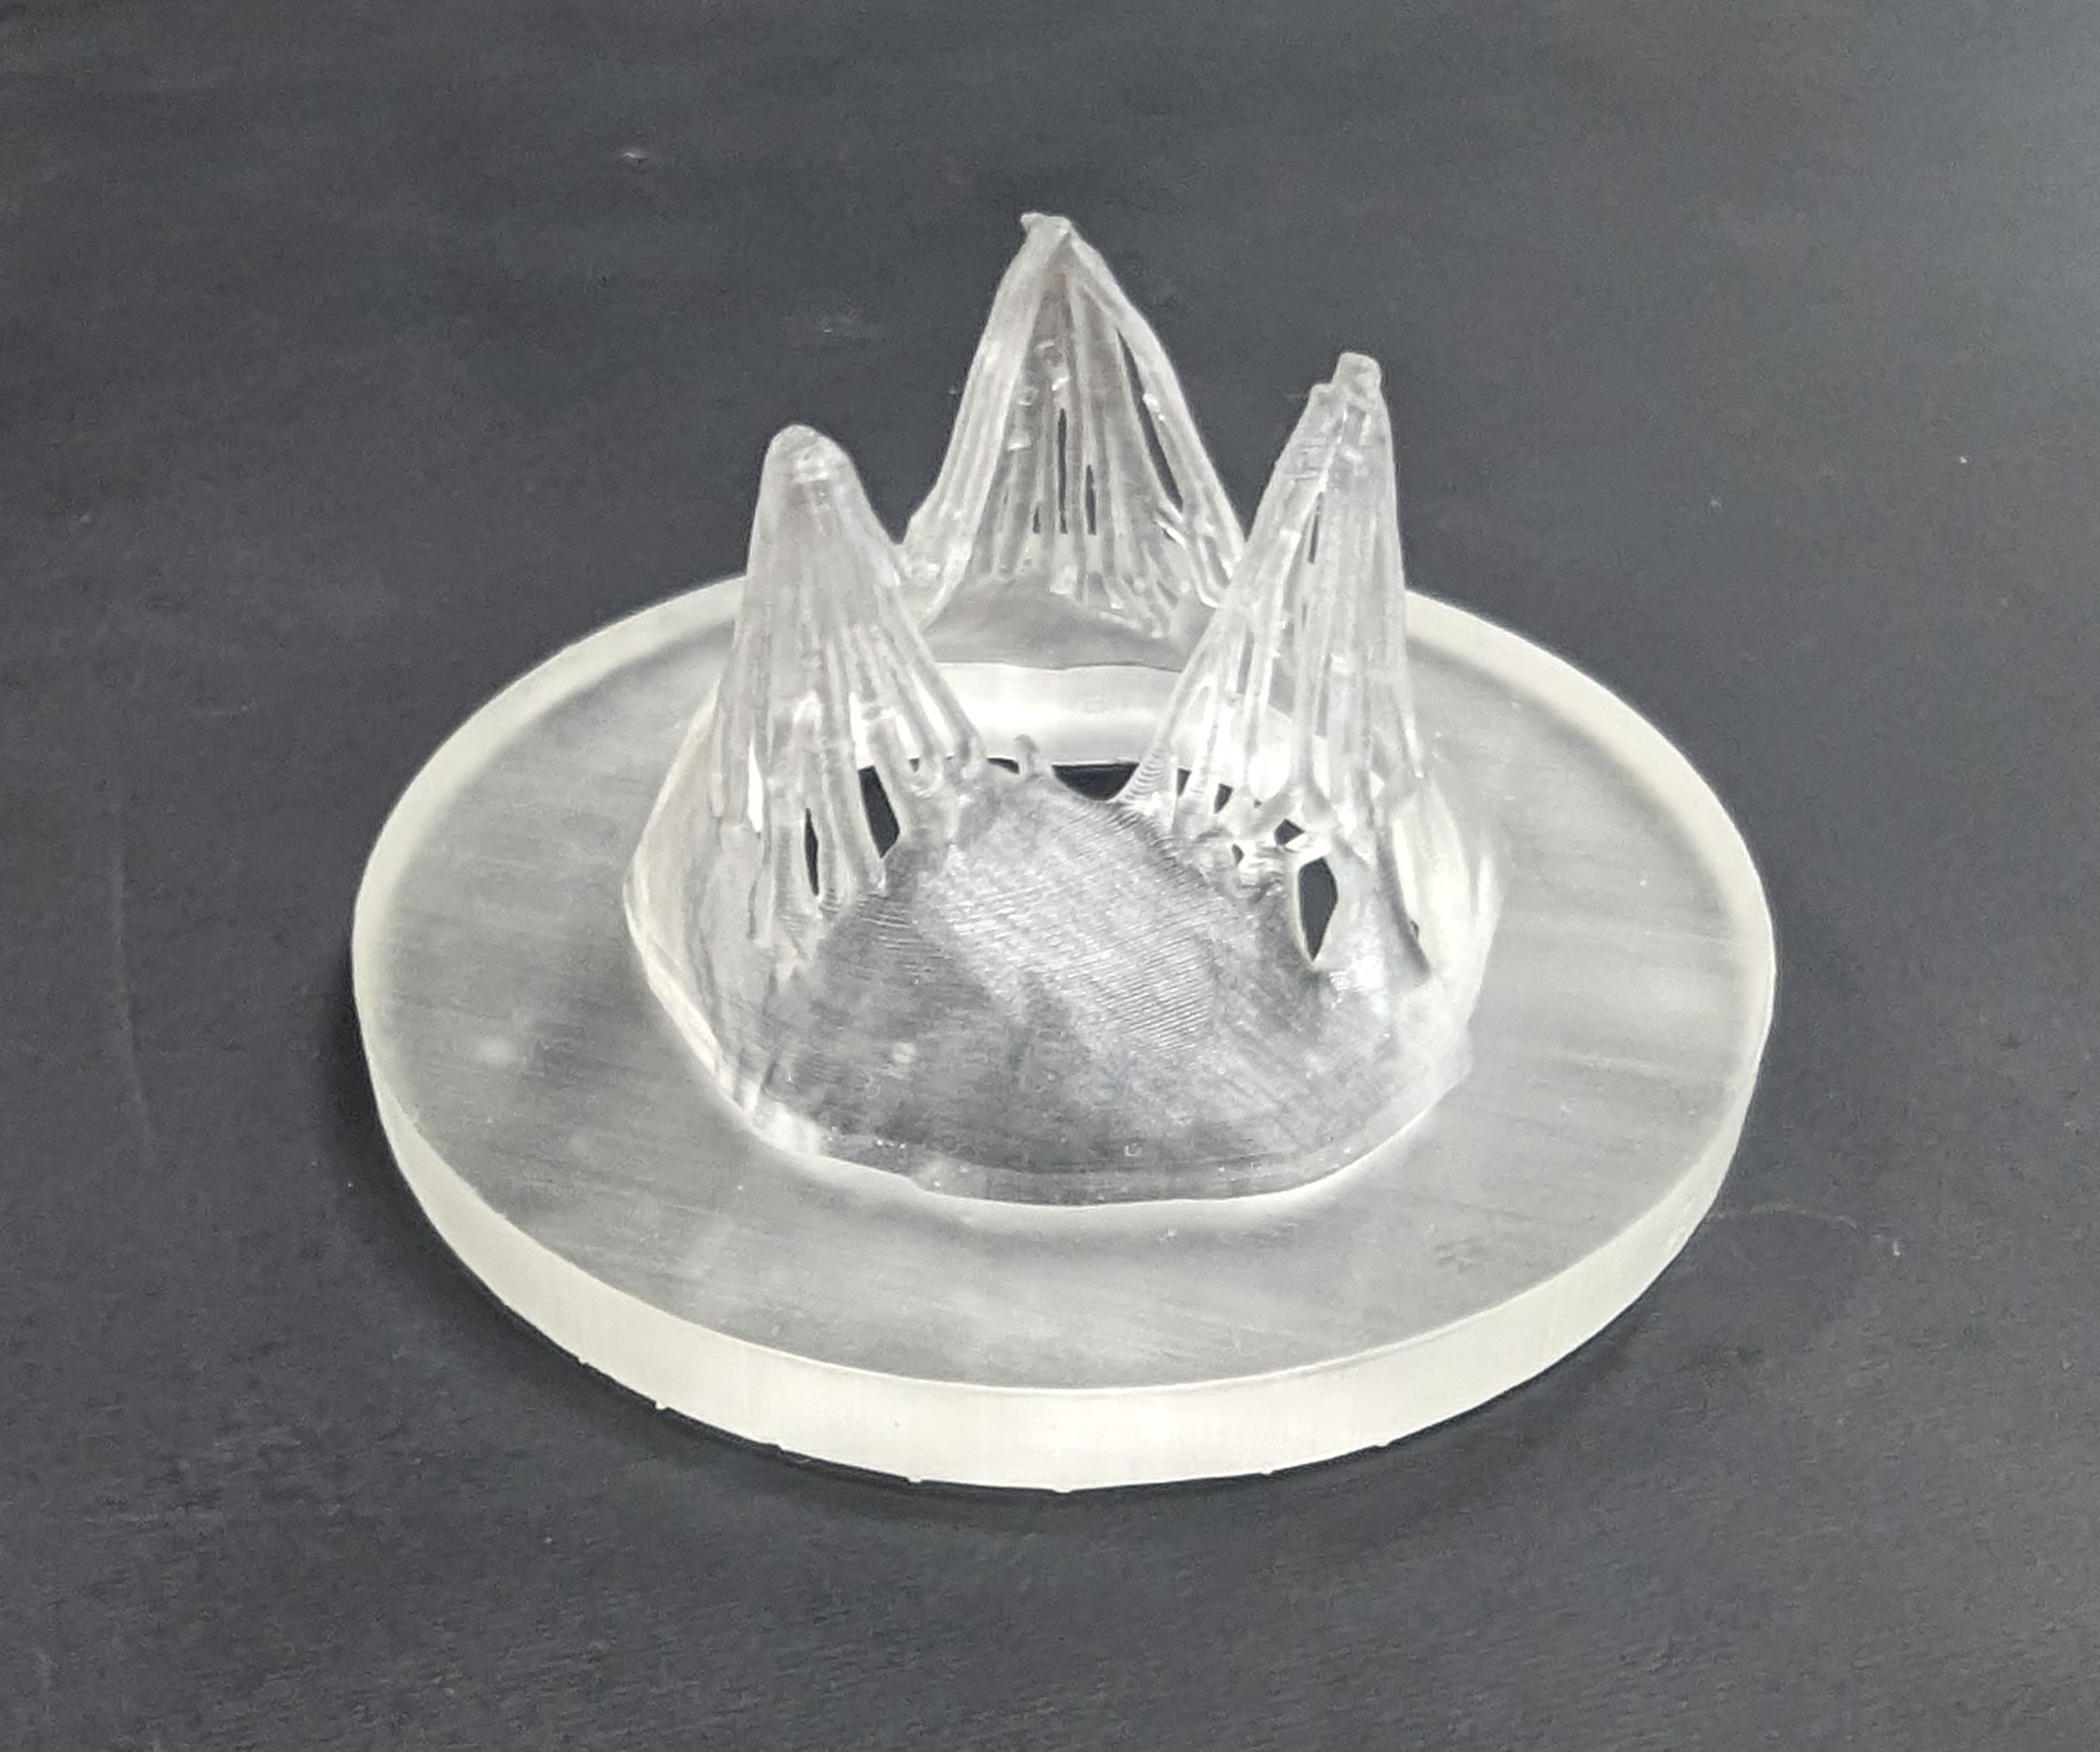
\includegraphics[width=0.75\textwidth]{figures/resinprintanat.jpg}
    \caption{Early revision SLA print of anatomical valve}
    \label{fig:reso}
\end{figure}
\marginpar{\textbf{Resources:}
    \begin{itemize}
        \item \href{https://help.prusa3d.com/article/faq-frequently-asked-questions_1932}{Prusa TDS}
        \item \href{https://formlabs.com/blog/understanding-accuracy-precision-tolerance-in-3d-printing/}{FormLabs TDS}
    \end{itemize}
}
\begin{itemize}
    \item The vastly increased tolerance of resin printing making parts much more accurate\\
          Prusa \gls{FDM}:0.3mm\\
          FormLabs \gls{SLA}:0.01mm
    \item The reduced layer height that resin printing is capable of\\
          Prusa \gls{FDM}:0.05mm\\
          FormLabs \gls{SLA}:0.025mm
\end{itemize}
This has two main benefits regarding this study;
\begin{itemize}
    \item Minimizing layer height results in mould parts reducing surface affects
    \item Reducing adhesion of cast part to mould, this is minimized on \gls{PLA} parts with mould release and sanding however with casted parts on this degree of thickness there can still be an increased risk of breakage in the demoulding process.
\end{itemize}
Another option worth considering is machining from either steel or a performance plastic like delrin \citeonly{liProcessOptimizationInmold2022}; this would be more expensive however, it could be worth the cost for moulds that need to be used for many castings as well as increasing the precision over multiple casts since 3D printed parts warp under the pressure of the clamping.

The importance of transparency for the part was a consideration for further work on the valve as the integration into the right heart simulator would involve \gls{PIV} measurement where maintaining transparency would allow for a measured flow field uninterrupted by the leaflets, this was an issue in studies like \citeonly{rabbahNovelLeftHeart2013} and the efficacy on dynamic transparent parts in \gls{PIV} rigs has been shown in studies like \citeonly{busenDevelopmentVitroPIV2017}.

\section{Contextualizing Results}

% Discuss how your results relate to previous studies and theoretical frameworks. Are your findings consistent with other studies, or do they diverge?
% Analyze the significance of any discrepancies and explore possible reasons.

The results of this study have shown how the development of imitative synthetic heart valves can be a valuable tool in cardiac simulators. The coaptation tests on the valve show great promise for a technology of this nature, surpassing limitations of previous work in simulational studies such as \citeonly{rabbahNovelLeftHeart2013} dissected porcine valves, \citeonly{gintyModelingPatientSpecificDeformable2018} rigid valves and \citeonly{raghavExperimentalAssessmentFlow2018} non-anatomically representative valves, Each have major limitations in their ability for a wider range of experiments.\\
Some such limitations of these valves are;
\begin{itemize}
    \item The longevity of porcine for repeated experiments. While it can be stored in the likes of formalin the tissue degrades over time which leads to an irrepeatability in testing and eventual need for replacement.
    \item Semi-rigid valves can't be used in flow studies as they can't deform to coapt.
    \item Non-anatomical valves can coapt but don't represent true geometry, which won't yield accurate results.
\end{itemize}
\subsection{Design Validation Testing}
The thickness testing of the casted and \gls{CAD} models gives a good idea of shrinkage percentages of the \gls{PU} material used and also discrepancies added from the process of tethering the nylon wire for chordae tendineae, these parameters are important as for computational studies being conducted in tandem require precise geometries. The results show a ~5\% shrinkage in the material which could make a significant difference.

There are however some limitations that limit the strength of these results. Micrometres have a measurement force of 0.5-2N, which acts on the leaflets as the gauge is tightened. While low, this force is enough to deform the leaflets slightly, leading to small but noticeable discrepancies in the results. Using a laser micrometre would be a good solution to this as it would allow for non-contact measurement of the thickness of the leaflets in much more precise locations; combining this with an adjustable platform to seat the valve in would yield much more accurate and perfectly repeatable results to assess shrinkage.

The locations of measurements were purposefully chosen to overlap with the attached tendineae as much as possible to assess their added thickness, this disruption to the geometry is not ideal as the surface acts much less predictably and be replicated in \gls{CAD} models since it is done by hand.


\subsection{Coaptation Testing}
\newthought{Chordae Tendineae Performacnce:}\\
The coaptation test illustrated how the chordae tendineae can be used in a synthetic part to prevent prolapse and aid coaptation. The aligns well with how it had been done before such as in \citeonly{rabbahNovelLeftHeart2013} and \citeonly{karlExvivoInvitroDynamic2024} where native and synthetic tendineae were used respectively. Such works also show how this part of the model can be manipulated with motors to simulate the contraction of papillary muscles, which while not applicable to the current design of the right heart simulator, could be developed for future iterations or simpler rig designs like that of the tube-based coaptation test \cref{fig:Videos}

\newthought{Leaflet Performance:}\\
The area with the most room for improvement is likely the leaflets. The final iteration from this study came very far relative to the initial iterations in terms of rigidity, transparency and geometric precision, it also performed better than similar attempts from other studies like \citeonly{gintyModelingPatientSpecificDeformable2018} although in regards to the initial design criteria from section:\cref{sec:Design Criteria}  it is lacking in functional performance and scalability

Not all the leaflets coapted together, which was the objective, however, it was supposed to occur from annular dilation and chordal loosening, not from the geometry not allowing it, this is most likely due to the model of the valve being based on a valve in the diastolic phase, so the full length of the leaflets were malformed in \gls{CT} conversion as they were not under load from the pressure systolic pressure which would stretch to there full length. This can be seen in \cref{fig:Videos}:B, where the leaflets move back but are not long enough to meet each other. The work of \citeonly{karlExvivoInvitroDynamic2024} capture this well in their mitral valve design, they did well with leaflet length however theyre design was not anatomically representative, building off this to capture both physiological replicity and functional performance would be a first of it's kind for in-vitro tricuspid valve testing.




